\documentclass{article}
\usepackage{enumerate}
\usepackage{amsmath}
\usepackage{amssymb}
\usepackage{graphicx}
\usepackage{subfigure}
\usepackage{geometry}
\usepackage{color}
\usepackage{bm}
\usepackage{indentfirst}
\usepackage{array}
\usepackage{multirow}
\usepackage{diagbox}
\usepackage{enumerate}
\usepackage{mathpazo} 
\usepackage{indentfirst}
\usepackage{amssymb}
\usepackage{helvet}
\usepackage{amsmath}
\usepackage{geometry}   
\usepackage{booktabs}
\usepackage{gensymb}
\usepackage{epsfig}
\usepackage{graphicx}
\usepackage{subfigure}  
\usepackage{float} 
\usepackage{multirow}
\usepackage{booktabs}
\usepackage{listings}
\usepackage{xcolor}
\usepackage{url}
\lstset{
 columns=fixed,       
 numbers=left,                                        % 在左侧显示行号
 numberstyle=\tiny\color{gray},                       % 设定行号格式
 frame=none,                                          % 不显示背景边框
 backgroundcolor=\color{white},            % 设定背景颜色
 keywordstyle=\color[RGB]{40,40,255},                 % 设定关键字颜色
 numberstyle=\footnotesize\color{black},           
 commentstyle=\it\color[RGB]{0,96,96},                % 设置代码注释的格式
 stringstyle=\rmfamily\slshape\color[RGB]{128,0,0},   % 设置字符串格式
 showstringspaces=false,                              % 不显示字符串中的空格
 language = verilog,                                        % 设置语言
}

\begin{document}

\vspace{0.4cm}

\hrulefill

\thispagestyle{empty}

\begin{center}
\begin{large}
\sc{UM--SJTU Joint Institute \vspace{0.3em} \\ Introduction to Computer Organization \\(VE370)}
\end{large}

\hrulefill

\vspace*{5cm}


\vspace{2em}

\begin{large}
\sc{{Project 2 Individual Report
\vspace{0.5em}


}}
\end{large}
\end{center}


\vfill

\begin{table}[h!]
\flushleft
\begin{tabular}{lll}

Zhan Yuhong\hspace*{2em}&
ID: 518021910565\hspace*{2em}\\

\\

Date: \today 

\end{tabular}
\end{table}


\newpage





\section{Introduction}

In Project 2, we are required to model a single cycle processor in Verilog HDL. I use the MIPS assembly program provided by TAs to verify that the processor can execute those instructions continuously and correctly.

\begin{figure}[H]
    \centering
    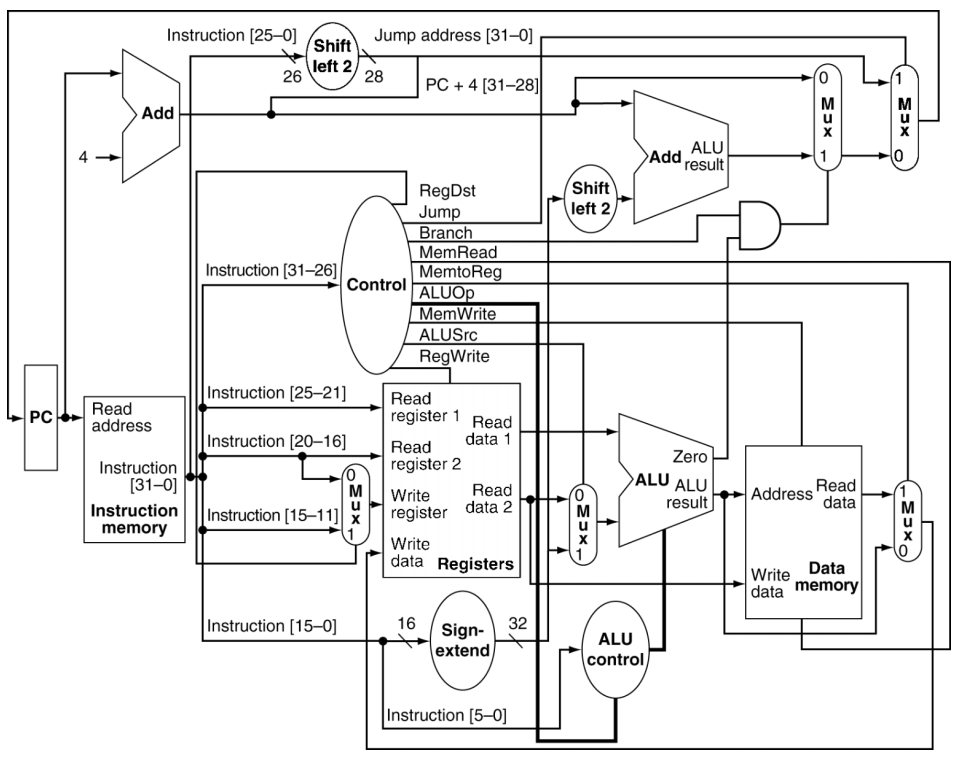
\includegraphics[height = 13cm,width = 16cm]{single_cycle.png}
    \caption{Single cycle implementation of MIPS architecture$^{[1]}$}
    \label{fig:my_label}
\end{figure}

The graph above is the single cycle implementation of MIPS architecture, but there are some extra MIPS instructions added such as "andi" "bne".

\section{Screen shots of simulation results for each type of instruction}

\subsection{addi \$t0, \$zero, 0x20}

\begin{figure}[H]
    \centering
    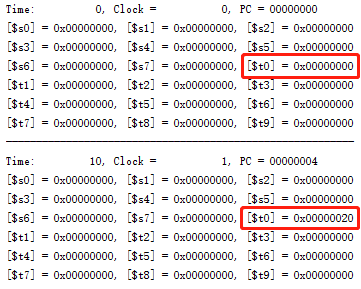
\includegraphics[height = 10cm,width = 13cm]{addi.png}
    \caption{addi}
    \label{fig:my_label}
\end{figure}

addi \$t0, \$zero, 0x20 \\

\subsection{and \$s0, \$t0, \$t1}

\begin{figure}[H]
    \centering
    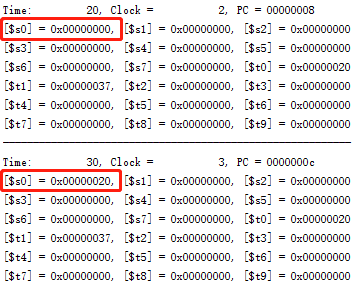
\includegraphics[height = 10cm,width = 13cm]{and.png}
    \caption{and}
    \label{fig:my_label}
\end{figure}

and \$s0, \$t0, \$t1

\subsection{or \$s0, \$t0, \$t1}
\begin{figure}[H]
    \centering
    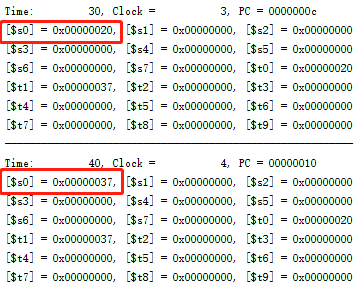
\includegraphics[height = 10cm,width = 13cm]{or.png}
    \caption{or}
    \label{fig:my_label}
\end{figure}

or \$s0, \$t0, \$t1
\subsection{sw \$s0, 4(\$zero)}
\begin{figure}[H]
    \centering
    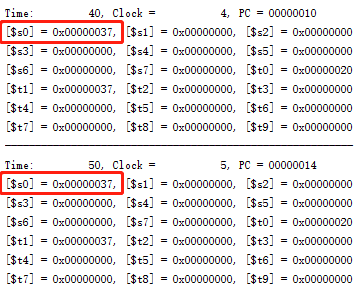
\includegraphics[height = 10cm,width = 13cm]{sw.png}
    \caption{sw}
    \label{fig:my_label}
\end{figure}

sw \$s0, 4(\$zero) \\

Since I don't display the content of data memory, the result of sw instruction should be showed in the following lw part.

\subsection{lw \$s1, 4(\$zero)}
\begin{figure}[H]
    \centering
    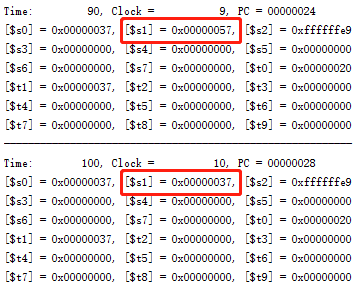
\includegraphics[height = 10cm,width = 13cm]{lw.png}
    \caption{lw}
    \label{fig:my_label}
\end{figure}

lw \$s1, 4(\$zero)
\subsection{add \$s1, \$t0, \$t1}
\begin{figure}[H]
    \centering
    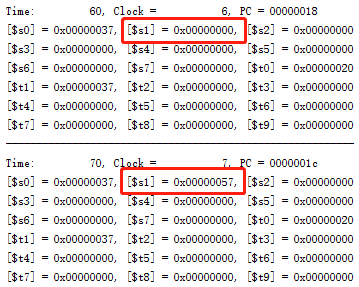
\includegraphics[height = 10cm,width = 13cm]{add.png}
    \caption{add}
    \label{fig:my_label}
\end{figure}
add \$s1, \$t0, \$t1

\subsection{sub \$s2, \$t0, \$t1}
\begin{figure}[H]
    \centering
    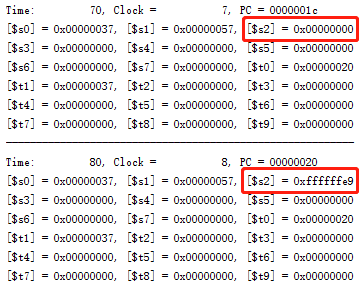
\includegraphics[height = 10cm,width = 13cm]{sub.png}
    \caption{sub}
    \label{fig:my_label}
\end{figure}

sub \$s2, \$t0, \$t1
\subsection{beq \$s1, \$s2, error0 (not branch)}
\begin{figure}[H]
    \centering
    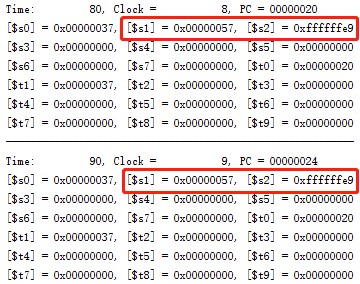
\includegraphics[height = 10cm,width = 13cm]{beq_not.png}
    \caption{beq (not branch)}
    \label{fig:my_label}
\end{figure}
beq \$s1, \$s2, error0

\subsection{andi \$s2, \$s1, 0x48}
\begin{figure}[H]
    \centering
    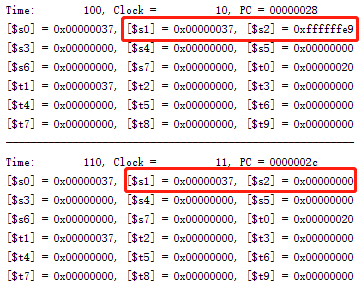
\includegraphics[height = 10cm,width = 13cm]{andi.png}
    \caption{andi}
    \label{fig:my_label}
\end{figure}
andi \$s2, \$s1, 0x48

\subsection{slt \$s4, \$s2, \$s1 (Last)}
\begin{figure}[H]
    \centering
    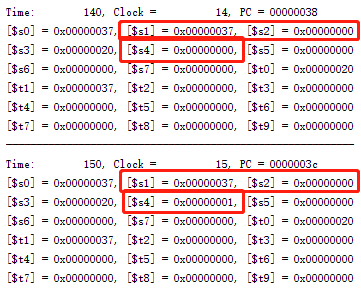
\includegraphics[height = 10cm,width = 13cm]{slt.png}
    \caption{slt}
    \label{fig:my_label}
\end{figure}
slt \$s4, \$s2, \$s1 (Last)

\subsection{j Last}
\begin{figure}[H]
    \centering
    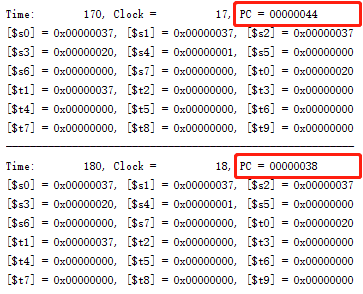
\includegraphics[height = 10cm,width = 13cm]{j.png}
    \caption{j}
    \label{fig:my_label}
\end{figure}

j Last

\subsection{beq \$s4, \$0, EXIT (branch)}
\begin{figure}[H]
    \centering
    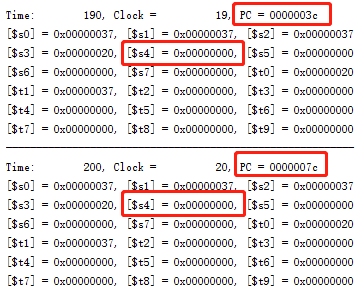
\includegraphics[height = 10cm,width = 13cm]{beq.png}
    \caption{beq (branch)}
    \label{fig:my_label}
\end{figure}

beq \$s4, \$0, EXIT

\subsection{bne $s0, $t0, EXIT (not branch)}

\begin{figure}[H]
    \centering
    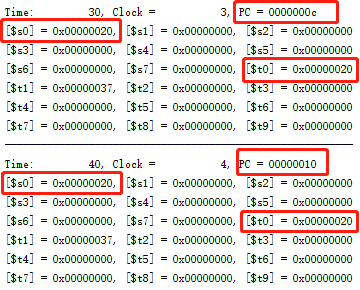
\includegraphics[height = 10cm,width = 13cm]{bne_not.png}
    \caption{bne (not branch)}
    \label{fig:my_label}
\end{figure}

bne \$s0, \$t0, EXIT

\subsection{bne $s0, $t0, EXIT (branch)}

\begin{figure}[H]
    \centering
    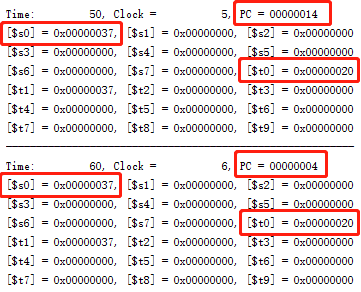
\includegraphics[height = 10cm,width = 13cm]{bne.png}
    \caption{bne (branch)}
    \label{fig:my_label}
\end{figure}

bne \$s0, \$t0, EXIT


\section{Testcase}

\subsection{single\_bonus.txt (addi to beq)}

\begin{lstlisting}
00100000000010000000000000100000 //addi $t0, $zero, 0x20
00100000000010010000000000110111 //addi $t1, $zero, 0x37
00000001000010011000000000100100 //and $s0, $t0, $t1
00000001000010011000000000100101 //or $s0, $t0, $t1
10101100000100000000000000000100 //sw $s0, 4($zero)
10101100000010000000000000001000 //sw $t0, 8($zero)
00000001000010011000100000100000 //add $s1, $t0, $t1
00000001000010011001000000100010 //sub $s2, $t0, $t1
00010010001100100000000000001001 //beq $s1, $s2, error0
10001100000100010000000000000100 //lw $s1, 4($zero)
00110010001100100000000001001000 //andi $s2, $s1, 0x48
00010010001100100000000000001001 //beq $s1, $s2, error1
10001100000100110000000000001000 //lw $s3, 8($zero)
00010010000100110000000000001010 //beq $s0, $s3, error2
00000010010100011010000000101010 //slt $s4, $s2, $s1 (Last)
00010010100000000000000000001111 //beq $s4, $0, EXIT
00000010001000001001000000100000 //add $s2, $s1, $0
00001000000000000000000000001110 //j Last
00100000000010000000000000000000 //addi $t0, $0, 0(error0)
00100000000010010000000000000000 //addi $t1, $0, 0
00001000000000000000000000011111 //j EXIT
00100000000010000000000000000001 //addi $t0, $0, 1(error1)
00100000000010010000000000000001 //addi $t1, $0, 1
00001000000000000000000000011111 //j EXIT
00100000000010000000000000000010 //addi $t0, $0, 2(error2)
00100000000010010000000000000010 //addi $t1, $0, 2
00001000000000000000000000011111 //j EXIT
00100000000010000000000000000011 //addi $t0, $0, 3(error3)
00100000000010010000000000000011 //addi $t1, $0, 3
00001000000000000000000000011111 //j EXIT
\end{lstlisting}

\subsection{single\_bne.txt (bne)}

\begin{lstlisting}
00100000000010000000000000100000 //addi $t0, $zero, 0x20
00100000000010010000000000110111 //addi $t1, $zero, 0x37 (EXIT)
00000001000010011000000000100100 //and $s0, $t0, $t1
00010110000010001111111111111101 //bne $s0, $t0, EXIT
00000001000010011000000000100101 //or $s0, $t0, $t1
00010110000010001111111111111011 //bne $s0, $t0, EXIT
\end{lstlisting}

\section{Peer evaluation}

\begin{table}[H]
\centering
\begin{tabular}{|c|c|c|}
\hline
Name & Level of contribution & Description of contribution \\ \hline
Yuhong Zhan & 5 & \begin{tabular}[c]{@{}c@{}}FPGA implementation, Debug Pipelined blocks,\\ Proofread team report\end{tabular} \\ \hline
Chenfzhang Lin & 5 & Debug Pipelined blocks, Write team report \\ \hline
Ruge Xu & 5 & \begin{tabular}[c]{@{}c@{}}FPGA implementation, Write team report,\\ Debug Pipelined blocks\end{tabular} \\ \hline
Yipeng Lin & 5 & Design Pipelined blocks, Debug Pipelined blocks \\ \hline
\end{tabular}
\caption{Peer evaluation}
\label{tab:my-table}
\end{table}
\newpage
\section{Reference}
[1]Zheng Gang, Ve370 Introduction to Computer Organization Project 2. 2020.11.12 \\

[2]IEEE Computer Society, Design Automation Standards Committee, IEEE Standard Verilog 

Hardware Description Language, The Institute of Electrical and Electronics Engineers, Inc. 3 

Park Avenue, New York, NY 10016-5997, USA. 28 September 2001.

\newpage

\section{Appendix}

\subsection{Verilog source files}

\begin{lstlisting}
`timescale 1ns / 1ps

module single_cycle(clk);
    input clk;
    wire RegDst, beq, bne, jump, MemRead, MemtoReg, MemWrite, ALUSrc, 
    RegWrite, zero, Branch;
    wire [1:0] ALUop;
    wire [3:0] ALUcontrol;
    wire [4:0] Write_reg;
    wire [31:0] PC_in, PC_out, instruction, PC_next, jump_addr, branch_addr, 
    Read_data1, Read_data2, Write_data, sign_extend, ALU_in, ALU_result, Read_data, 
    Add1, Add2, branch_out;
    
    assign jump_addr = {Add1[31:28], instruction[25:0], 2'b00};

    Add add1(PC_out, 4, Add1);
    Add add2(Add1, sign_extend * 4, Add2);
    
    Mux_2to1 #(32) branch(((beq && zero) | (bne && ~zero)), Add1, Add2, branch_out);
    Mux_2to1 #(32) Jump(jump, branch_out, jump_addr, PC_in); 
    Mux_2to1 #(5) write_reg(RegDst, instruction[20:16], instruction[15:11], Write_reg);
    Mux_2to1 #(32) ALUin(ALUSrc, Read_data2, sign_extend, ALU_in);
    Mux_2to1 #(32) write_data(MemtoReg, ALU_result, Read_data, Write_data);  
    
    PC pc(clk, PC_in, PC_out);    
    Ins_memory IM(PC_out, instruction);
    Control control(instruction[31:26], RegDst, beq, bne, jump, MemRead, 
    MemtoReg, MemWrite, ALUop, ALUSrc, RegWrite);      
    Registers Reg_file(clk, RegWrite, instruction[25:21], instruction[20:16], 
    Write_reg, Write_data, Read_data1, Read_data2);
    Sign_extend sign(instruction[15:0], sign_extend);
    ALU_control ALUctrl(ALUop, instruction[5:0], ALUcontrol);
    ALU alu(Read_data1, ALU_in, ALUcontrol, zero, ALU_result);
    Data_memory datamem(clk, MemRead, MemWrite, ALU_result, Read_data2, Read_data);
endmodule

module Add(a, b, sum);
    input [31:0] a, b;
    output reg [31:0] sum;
    always @ (*) begin
        sum = a + b;
    end 
endmodule

module Mux_2to1(sel, data1, data2, result);
    parameter N = 32;
    input sel;
    input [N - 1:0] data1, data2;
    output reg [N - 1:0] result;
    always @ (*) begin
        result = (sel == 0) ? data1:data2;
    end
endmodule

module PC(clk, PC_in, PC_out);
    input clk;
    input [31:0] PC_in;
    output reg [31:0] PC_out;
    initial begin
        PC_out = 0;
    end
    always @ (posedge clk) begin
        PC_out <= PC_in;
    end
endmodule

module Ins_memory(Read_addr, Instruction);
    input [31:0] Read_addr;
    output reg [31:0] Instruction;
    reg [31:0] ins_memory [63:0];
    integer i;
    initial begin 
        for (i = 0; i < 64; i = i + 1) ins_memory[i] = 0;
        $readmemb("E:/zhan/VE370/Project/Project2/single_bonus.txt", ins_memory);
    end
    always @ (Read_addr) begin
        Instruction = ins_memory[Read_addr/4];
    end
    //assign Instruction = ins_memory[Read_addr/4];
endmodule

module Control(op, RegDst, beq, bne, jump, MemRead, MemtoReg, MemWrite, ALUop, 
ALUSrc, RegWrite);
    input [5:0] op;
    output reg RegDst, beq, bne, jump, MemRead, MemtoReg, MemWrite, ALUSrc, RegWrite;
    output reg [1:0] ALUop;
    initial begin
        RegDst = 0;
        beq = 0;
        bne = 0;
        jump = 0; 
        MemRead = 0; 
        MemtoReg = 0; 
        MemWrite = 0;
        ALUSrc = 0;
        RegWrite = 0;
        ALUop = 0;
    end
    always @ (op) begin
        case (op)
            // R
            6'b000000: begin 
                RegDst <= 1;
                beq <= 0;
                bne <= 0;
                jump <= 0; 
                MemRead <= 0; 
                MemtoReg <= 0; 
                MemWrite <= 0;
                ALUSrc <= 0;
                RegWrite <= 1;
                ALUop <= 2'b10;
            end
            // j
            6'b000010: begin 
                RegDst <= 0;
                beq <= 0;
                bne <= 0;
                jump <= 1; 
                MemRead <= 0; 
                MemtoReg <= 0; 
                MemWrite <= 0;
                ALUSrc <= 0;
                RegWrite <= 0;
                ALUop <= 2'b10;
            end
            // beq
            6'b000100: begin 
                RegDst <= 0;
                beq <= 1;
                bne <= 0;
                jump <= 0; 
                MemRead <= 0; 
                MemtoReg <= 0; 
                MemWrite <= 0;
                ALUSrc <= 0;
                RegWrite <= 0;
                ALUop <= 2'b01;
            end
            // bne
            6'b000101: begin 
                RegDst <= 0;
                beq <= 0;
                bne <= 1;
                jump <= 0; 
                MemRead <= 0; 
                MemtoReg <= 0; 
                MemWrite <= 0;
                ALUSrc <= 0;
                RegWrite <= 0;
                ALUop <= 2'b01;
            end
            // addi
            6'b001000: begin 
                RegDst <= 0;
                beq <= 0;
                bne <= 0;
                jump <= 0; 
                MemRead <= 0; 
                MemtoReg <= 0; 
                MemWrite <= 0;
                ALUSrc <= 1;
                RegWrite <= 1;
                ALUop <= 2'b00;
            end 
            // andi
            6'b001100: begin 
                RegDst <= 0;
                beq <= 0;
                bne <= 0;
                jump <= 0; 
                MemRead <= 0; 
                MemtoReg <= 0; 
                MemWrite <= 0;
                ALUSrc <= 1;
                RegWrite <= 1;
                ALUop <= 2'b11;
            end
            // lw
            6'b100011: begin 
                RegDst <= 0;
                beq <= 0;
                bne <= 0;
                jump <= 0; 
                MemRead <= 1; 
                MemtoReg <= 1; 
                MemWrite <= 0;
                ALUSrc <= 1;
                RegWrite <= 1;
                ALUop <= 2'b00;
            end
            // sw
            6'b101011: begin 
                RegDst <= 0;
                beq <= 0;
                bne <= 0;
                jump <= 0; 
                MemRead <= 0; 
                MemtoReg <= 0; 
                MemWrite <= 1;
                ALUSrc <= 1;
                RegWrite <= 0;
                ALUop <= 2'b00;
            end                                                
        endcase
    end
endmodule

module Registers(clk, RegWrite, Read_reg1, Read_reg2, Write_reg, Write_data, 
Read_data1, Read_data2);
    input clk, RegWrite;
    input [4:0] Read_reg1, Read_reg2, Write_reg;
    input [31:0] Write_data;
    output [31:0] Read_data1, Read_data2;
    reg [31:0] memory [31:0];
    integer i;
    initial begin 
        for (i = 0; i < 32; i = i + 1)
            memory[i] = 0;
    end
    assign Read_data1 = memory[Read_reg1];
    assign Read_data2 = memory[Read_reg2];
    always @ (posedge clk) begin
        if (RegWrite == 1)
            memory[Write_reg] <= Write_data;
        end
endmodule

module Sign_extend(in, out);
    input [15:0] in;
    output [31:0] out;
    assign out = {{16{in[15]}},in};
endmodule

module ALU_control(ALUop, funct, out_control);
    input [1:0] ALUop;
    input [5:0] funct;
    output reg [3:0] out_control;
    always @ (*) begin
        case(ALUop)
            // lw, sw, addi
            2'b00: out_control = 4'b0010; // add
            // beq and bne
            2'b01: out_control = 4'b0110; // subtract
            // R-type
            2'b10: begin
                case (funct)
                    6'b100000: out_control = 4'b0010; // add
                    6'b100010: out_control = 4'b0110; // subtract
                    6'b100100: out_control = 4'b0000; // and
                    6'b100101: out_control = 4'b0001; // or
                    6'b101010: out_control = 4'b0111; // stl
                endcase
            end
            // andi
            2'b11: out_control = 4'b0000; // and
        endcase
    end
endmodule

module ALU(a, b, control, zero, result);
    input [31:0] a, b;
    input [3:0] control;   
    output zero;
    output reg [31:0] result;
    initial begin
        result = 0;
    end
    always @ * begin
        case (control)
            4'b0000: result = a & b;
            4'b0001: result = a | b;
            4'b0010: result = a + b;
            4'b0110: result = a - b;
            4'b0111: begin
                if (a < b)
                    result = 1;
                else
                    result = 0;
            end
            4'b1100: result = ~(a | b);
        endcase
    end
    assign zero = (result) ? 0 : 1;    
endmodule

module Data_memory(clk, MemRead, MemWrite, addr, Write_data, Read_data);
    input clk, MemRead, MemWrite;
    input [31:0] addr, Write_data;
    output [31:0] Read_data;
    reg [31:0] memory [63:0];
    integer i;
    initial begin
        for (i = 0; i < 64; i = i + 1)
            memory[i] = 0;
    end
    always @ (addr) begin
        if (MemWrite) memory[addr / 4] = Write_data;
    end
    assign Read_data = (MemRead) ? memory[addr / 4] : 0;
endmodule

\end{lstlisting}

\end{document}
